\chapter{The socio-technical system of \textit{core} projects}
\chaptermark{``Mostly-online" contributions: \textit{core} projects}
\label{chapter:core-system}

This chapter continues the exploration of different socio-technical systems of contribution activities, focussing on the development of \textit{core} projects. As previously discussed, these \textit{core} projects represent the heart of Drupal: its main codebase providing basic functionalities. Technically, they represent the highest degree of complexity and interdependency within the Drupal project.

The forthcoming sections show how the general organisational processes of this socio-technical system of contribution were also subjected to dynamics of formalisation and decentralisation. The degree of formalisation achieved in this socio-technical system is the highest of those found for ``mostly-online" contribution activities. The trend over time in relation to decision-making has also tended towards decentralisation, although to a lesser extent and resulting in a socio-technical system of contribution with a lower degree of autonomy than that of \textit{contributed} projects.

Following a structure similar to that seen in the previous chapter, section \ref{subsec:dries-beginning} provides an overview of the emergence of this socio-technical system, discussing the significant differences found compared to that of \textit{contributed} projects. In the next two subsections, the focus will be placed on the changes experienced during the transition from Drupal 7 to Drupal 8, comprising five of the fifteen years of Drupal's life, and in which the growth of contributors was especially significant. Section \ref{subsec:dec-form-core} explores general organisational aspects, showing how formalisation and decentralisation occurred at a more macro level, by exploring core initiatives, initiative leaders and core gates, among other organisational changes. Finally, a case study of one of these core initiatives --- ``Twig in Core" --- is presented in section \ref{subsec:dec-core-initiative}, in order to highlight how the aforementioned dynamics of formalisation and decentralisation operate at a more micro level.

\section{The emergence of the socio-technical system of \textit{core} projects: ``in the beginning was Dries"}
\label{subsec:dries-beginning}

In a similar way as in the socio-technical system of \textit{contributed} projects, the early organisational processes of \textit{core} projects were informal. For example, there were no explicit rules with regards to the governance of the project, nor a clear division of labour or attributions with the exception of the common BDFL\footnote{See previous footnote \ref{bdfl} for further details.} (Benevolent Dictator For Life) de-facto role of Dries. This is a role given to FLOSS development leaders, typically the founders of the project. It implicitly states that they retain the final word regarding conflicts and arguments in the community. The following excerpt from I\textunderscript{10} illustrates the informality of the self-organisational processes related to the development of core during the initial period:

\begin{quotation}
``[...] Once upon a time [he mentioned later `up to somewhere between Drupal 5 and 6' (2006-2008)] the process was: [...] Dries\footnote{As in the case of other studies on CBPP communities (e.g. \textcite{forte2009decentralization}) the name of the project founder becomes impractical, if not impossible, to anonymise. For these reasons, the name of Dries is used when referring to him in the interviews or excerpts from the field notes.} opens up a new branch, and the committers are Dries and a few of his old friends. Pretty much just him and \textit{Pete}, were the only ones who were active when I got involved. A new branch is open, people say: `Hey, I feel like working on X'. They go and work on X. When Dries feels it's ... feels about right, we have a code freeze, and then bang on [REMOVE] bugs, until we release a new version. And that process was maybe a year long cycle on average."
\begin{flushright}\footnotesize{Drupal core developer and architect, M, 11 years.}\end{flushright}
\end{quotation}

A similar key aspect as that discussed in section \ref{subsec:emergence-contrib} can be observed in this excerpt for the case of \textit{core} projects: the relevance and perceived value that having power to commit code or to create releases already had at the time. Early on in core, Dries was responsible for creating releases, and he and his friend were the only Drupalistas with the power to commit to core --- acting as gatekeepers for quality control. These powers to commit and create releases are also relevant to understand the decentralisation of decision-making with respect to the organisational processes in this system. However, while in the case of \textit{contributed} projects it led to the emergence of a system in which the power was more distributed and with a higher degree of autonomy in the hands of project maintainers; in the case of core the power to create releases and commit code remained more centralised overall, although similar figures of maintainers would eventually emerge over time. This higher degree of centralisation is explained by Drupalistas as responding to the need to coordinate a larger and constantly growing number of contributors --- as previously depicted in figure \ref{core-committers-release} --- in comparison with the socio-technical system of \textit{contributed} projects, as well as in the inherent complexity of a larger codebase which is less decoupled. Figures \ref{core-modules-release} and \ref{loc-core} show the growth in number modules and number of lines of code in core respectively, providing indicators of this growth in the complexity of the object.

    % Plot for number of core projects per release
    \begin{figure}[H]
    \centering
     \begin{tikzpicture}
      \begin{axis}[width=12cm, date coordinates in=x,date ZERO=2001-01-01,
                   xticklabel=\year-\month-\day,ymin=0,ymax=75,
                   x tick label style={rotate=45, anchor=east, align=center, yshift=-5pt},
                   label style={font=\tiny},
           xmin=2001-01-01,
           xmax=2016-03-10]
       \addplot coordinates {
    (2001-01-15,18)
    (2001-03-15,22)
    (2001-09-15,26)
    (2002-06-15,27)
    (2003-02-01,28)
    (2003-08-01,30)
    (2003-11-01,31)
    (2004-04-01,30)
    (2004-10-18,32)
    (2005-04-15,32)
    (2006-05-01,31)
    (2007-01-15,29)
    (2008-02-13,34)
    (2011-01-05,41)
    (2015-11-19,64)
       };
       
\addplot[mark=*] coordinates {(2001-01-15,18)} node[pin=-30:{$(v1.0)$}]{} ;
\addplot[mark=*] coordinates {(2001-03-15,22)} node[pin=-25:{$(v2.0)$}]{} ;
\addplot[mark=*] coordinates {(2001-09-15,26)} node[pin=-20:{$(v3.0)$}]{} ;
\addplot[mark=*] coordinates {(2002-06-15,27)} node[pin=-268:{$(v4.0)$}]{} ;
\addplot[mark=*] coordinates {(2003-02-01,28)} node[pin={[pin distance=2cm]-15:{$(v4.1)$}}]{} ;
\addplot[mark=*] coordinates {(2003-08-01,30)} node[pin={[pin distance=2.5cm]-265:{$(v4.2)$}}]{} ;
\addplot[mark=*] coordinates {(2003-11-01,31)} node[pin=-272:{$(v4.3)$}]{} ;
\addplot[mark=*] coordinates {(2004-04-01,30)} node[pin={[pin distance=1cm]-10:{$(v4.4)$}}]{} ;
\addplot[mark=*] coordinates {(2004-10-18,32)} node[pin={[pin distance=2.5cm]270:{$(v4.5)$}}]{} ;
\addplot[mark=*] coordinates {(2005-04-15,32)} node[pin={[pin distance=3cm]-270:{$(v4.6)$}}]{} ;
\addplot[mark=*] coordinates {(2006-05-01,31)} node[pin= -270:{$(v4.7)$}]{} ;
\addplot[mark=*] coordinates {(2007-01-15,29)} node[pin=-30:{$(v5.0)$}]{} ;
\addplot[mark=*] coordinates {(2008-02-13,34)} node[pin=-30:{$(v6.0)$}]{} ;
\addplot[mark=*] coordinates {(2011-01-05,41)} node[pin=-30:{$(v7.0)$}]{} ;
\addplot[mark=*] coordinates {(2015-11-19,64)} node[pin=180:{$(v8.0)$}]{} ;   

    \legend{Number of \textit{core} projects per release}
    \end{axis}
    \end{tikzpicture}
        \caption[Number of \textit{core} projects per release]%
        {Number of \textit{core} projects per release. Based on data collected by \textcite{zoubi-history:2016:Online}. Retrieved \nth{10} March 2016, from \url{http://websolutions.hr/drupal-history}, under a CC BY-SA 2.0 license.}
        \label{core-modules-release}
    \end{figure}

\begin{figure}[H]
  \centering
   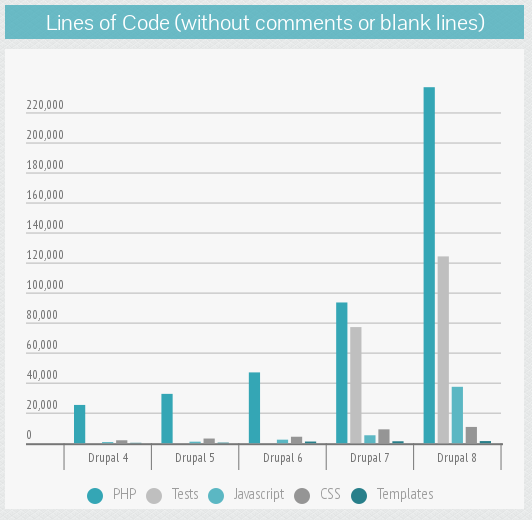
\includegraphics[scale=0.6]{graphs/lines_of_code_in_core}
   \caption[Number of lines of code in core per release]%
        {Number of lines of code in core (excluding comments and blank lines) for the latest five releases of Drupal, based on an infographic by \textcite{core-loc:2016:Online}. Retrieved \nth{10} March 2016, from \url{http://drupalmotion.com/article/drupal-code-base}.}
\label{loc-core}
\end{figure}

Nevertheless, the higher degree of centralisation cannot only be understood in technical terms, but also as intertwined with social aspects, such as the internal perceived greater value of contributing to Drupal core. Changes in Drupal core affect the global direction of the project and, as a consequence, they have also been subjected to higher degrees of quality assurance, while the power to carry out modifications in these digital commons have remained more centralised when compared to \textit{contributed} projects, and even more so when compared with \textit{custom} projects not shared within Drupal.org. This rigidity in the processes is also intertwined with a higher degree of legitimacy to carry out these changes, when compared with projects in the \textit{contributed} system and, consequently, an even higher degree when compared with the \textit{custom} system. The following quote by I\textunderscript{10} illustrates the idea of how being able to perform large modifications in core used to operate on the basis of trust generated around the informal network explained in the previous quote, and how changes required, and continue to require, a higher degree of legitimacy --- in the form of the approval of the project leader in this case:

\begin{quotation}
``[...] so I was sitting on the floor, in the party room [during DrupalCon Sunnyvale (2007)] that night. With this little netbook that I borrowed from the company [looking at documentation to propose a set of changes in core]. [...] And Dries comes by, sits down on the floor next to me. And... after I explained to him [the proposed changes] he said:  `Yes, this makes senses, go with it'. Wait... what, what? [LAUGHS]. [...] And, you know, at this point I think he knew who I was, because I had done enough bits and pieces over the last year or so. But, that kick in the pants to say: `OK, you have the project leader's blessing to do this big thing'. It was huge. And getting that... you know, a lot of people like to talk about Open Source: `You don't need permission to get involved', but you kind of do when you are doing it at a high level, when you are making large changes, you do need to have someone's blessing. [...] And that blessing did help."
\begin{flushright}\footnotesize{Drupal core developer and architect, M, 11 years.}\end{flushright}
\end{quotation}

Nevertheless, this does not imply that these processes were not affected by the general dynamics of formalisation and decentralisation previously described. A similar trend of decentralisation in decision-making could be observed over time as well, but this occurred in a more rigid environment, when compared with that of \textit{contributed} projects. The next quote, by I\textunderscript{9}, illustrates this increasing need to decentralise the decision-making processes --- most significantly during the transition from Drupal 7 to 8 --- due to the growth of the community, and its relationship to the increase in the degree of formalisation:

\begin{quotation}
``[...] And now, because it's so big and there's so many changes that there's no real way to do that informally. There needs to be a formal process, so that the people who are responsible for doing certain things know that they're responsible for it, and know how to get it done. And people know how to contact them to ask them to do these things that they are responsible for. So, it has been getting more explicit and better documented, just because the people who need to be doing these things, need to be able to do them [...] and that's because as we get bigger, and we have a reputation for helping people get involved with contributing to Open Source, we get a ton of new people who want to contribute."
\begin{flushright}\footnotesize{Drupal core developer and mentoring organiser, F, 8 years.}\end{flushright}
\end{quotation}

During the same interview, I\textunderscript{9} also explained how the trend towards increasing the degree of formalisation reached a higher degree than in the case of the \textit{contributed} system, which can be interpreted on the basis of these processes being subjected to the aforementioned higher degree of expected legitimacy as well as accountability to the community:

\begin{quotation}
``[...] So, the procedures have to be more formalised in order for it to be welcoming for new contributors. Because people need to know how we do things, who to talk to, and why. Otherwise, it looks like ... like you have to be part of the in-crowd, or you have to know certain people, or you have to be in a \textit{backchannel}, and that stuff is really bad. It will drive away new contributors. So the formalisation has definitely increased, and I think it's a really good thing. Both, for the people who have to do the things, so they realise what they have to do. We talk about how to do them, and we come to some kind of agreement and plan. And also, for the new people, so we aren't hiding anything. The information that they need in order to contribute is exposed to them."
\begin{flushright}\footnotesize{Drupal core developer and mentoring organiser, F, 8 years.}\end{flushright}
\end{quotation}

To further understand how the general dynamics of formalisation and decentralisation shaped the self-organisational processes related to the development of \textit{core} projects, the next sections will provide a more extensive description and analysis of key aspects. Following a structure similar to that of chapter \ref{sec:custom-to-contrib}, the focus will be placed firstly on how formalisation and decentralisation occurred in the general organisational aspects. With that goal in mind, the changes experienced in the transition between cores 7 to 8, the longest release period in the history of the community as well as with the highest number of contributors in terms of code committers, will be discussed. Secondly, a specific core initiative is presented and analysed, following a similar structure as in section \ref{subsec:contrib-day-by-day} for the case of \textit{contributed} projects, in order to illustrate how these changes in the general organisational aspects facilitated the empowering of part of the community to change the direction of the project.

\section{Core initiatives, leaders and gates: formalisation and decentralisation in core}
\label{subsec:dec-form-core}

While minor changes in \textit{core} projects are introduced via patches, the possibility to carry out large changes which affect the direction of the project are harder to achieve when compared to \textit{contributed} projects  and require a higher degree of legitimacy in the community. As illustrated in the previous section, in the early stages the process strongly depended on the closeness of an informal network. As the community continued to grow, these processes incorporated more formalised mechanisms to improve transparency, objectivity and monitoring of these peer-production processes. The most prominent examples of this formalisation can be found during the transition from Drupal 7 to Drupal 8 --- five years of development, a third of the life of Drupal --- , as I\textunderscript{8} explained:

\begin{quotation}
``[...] So Drupal 7 was released, and Drupal 8 was open for development. And Dries knew that he wasn't gonna be able to make decisions about everything. And there were a lot of big ideas, that he wanted to be changed for Drupal 8. So I think there were four or five big ideas, and he decided to pick initiative leads that would... like lead making those things happen. And then he could still be contacted for certain things, but initiative leads would have... the responsibility to organise, review, and maintain... to try to make these goals happen."
\begin{flushright}\footnotesize{Drupal core developer and mentoring organiser, F, 8 years.}\end{flushright}
\end{quotation}

These \textit{official} initiatives\footnote{See \url{https://www.drupal.org/node/2107085}.} entailed a significant increment in the degree of formalisation with respect to early stages --- including formal leaders, roadmaps and a reflection in the tools of the main collaboration platform (see figure \ref{core-initiative}).

\begin{figure}[H]
   \centering
   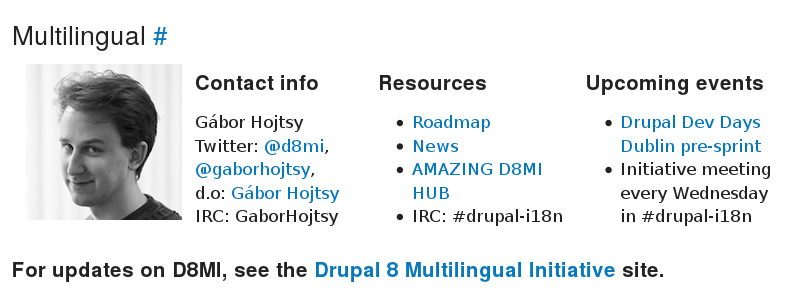
\includegraphics[scale=0.5]{img/online/core_initiative.png}
   \caption[Example of information about official core initiative in Drupal.org]%
   {Example of the information about an official core initiative in Drupal.org, in this case ``Multilingual". Retrieved \nth{20} April 2015, from \url{https://www.drupal.org/node/2107085}, under a CC BY-SA 2.0 license.}
\label{core-initiative}
\end{figure}

However, in congruence with the higher degree of centralisation in this socio-technical system of contribution, the process was still carried out in a prominent top-to-bottom way: based on the direct appointment of well-known Drupalistas by Dries. Although this initial step could be understood as a matter of simple delegation, it also opened up a large discussion about how these decisions should be made. For example, this was reflected in the creation of formal rules discussed by the community with regard to the governance of core \parencite{drupalorg-core-governance:2016:Online}, as well as a more formalised division of labour. The following quote by I\textunderscript{10} illustrates this dynamic of formalisation and its reflection in the division of labour (e.g. formal roles such as project owners, release managers or subsystem maintainers), rules (e.g. attributions of those roles and explicit governance of core) and artefacts (e.g. distribution of power to commit changes),  among others:

\begin{quotation}
``[...] And that triggered a very extensive debate, which sometimes got a bit more heated than it should have. But, in the end I think it was good to air some of those problems. So earlier that year, we pushed through a new formalised structure. [...] we have an actual release manager role. We have a... someone actively called a project owner, and that's Dries and \textit{Jane}. And we clarified what a subsystem maintainer can and cannot do, sort of. And there are people who are now specifically supposed to look after the big picture architecture: \textit{Roger} and \textit{Joe}. And give lots of those people commit access to help again keep the RTBC [Reviewed and Tested By the Community] queue short. [...] We are trying to increase the amount of structure.[...] You need to have, you know, local structures of control which are part of a larger picture."
\begin{flushright}\footnotesize{Drupal core developer and architect, M, 11 years.}\end{flushright}
\end{quotation}

Overall, this led to the definition of more clearly defined community boundaries, which also established more effective ways to provide modifications of the rules by those who are affected by them. In addition this trend shows how the individuals responsible for monitoring those commons, in accordance with collective-choice arrangements, were required to become more accountable to the community and transparency increased. The following excerpt, extracted from the personal blog of a core maintainer in the context of a discussion about contribution and influence, illustrates how these changes in the self-organisational processes operate on a day-to-day basis and their reflection in the artefacts:

\begin{figure}[H]
\centering
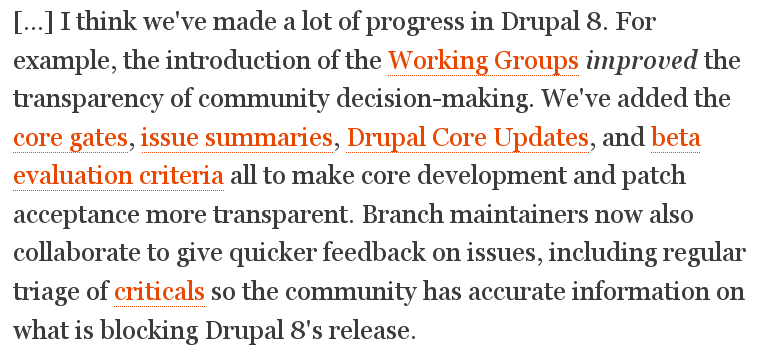
\includegraphics[scale=0.45]{img/quotes_replacement/contribution-influence-drupal-8.png}
\caption[Excerpt from the article ``Contribution, Influence, and Drupal 8"]{Drupal core maintainer, F, 8 years. Excerpt from the article ``Contribution, Influence, and Drupal 8". Retrieved \nth{11} March 2015, from \url{http://xjmdrupal.org/blog/contribution-influence-drupal-8}.}
\label{quote_core_influence}
\end{figure}

For example, the Core Gates \parencite{drupalorg-core-gates:2015:Online, drupalorg-core-gates-rfc:2015:Online}, to which the Drupalista referred, are essentially sets of ``checklists" in different areas such as performance, accessibility, documentation, usability and testing, which emerged in response to the need to define explicit quality assurance mechanisms in ways which these collective-choice arrangements can be created and modified by a wider amount of Drupalistas willing to participate. For instance, specific groups were created to participate in its elaboration. Each of them had long discussions joined by hundreds to thousands of participants, which varied depending on the specific gate \parencite{drupalorg-core-gates-testing:2015:Online, drupalorg-core-gates-performance:2015:Online, drupalorg-core-gates-accesiblity:2015:Online}. Furthermore, this process of formalisation facilitated decentralisation in the decision-making beyond \textit{official} initiatives\footnote{Further details on \textit{unofficial} initiatives are extensively discussed in section \ref{subsec:dec-core-initiative}.}. Overall, these changes illustrate how the possibility to perform large modifications in these digital commons, in other words the power to change the direction of the project, became more distributed and transited from depending on an informal network towards depending more on explicit sets of collective-choice arrangements discussed and formalised by the community. The following excerpt from I\textunderscript{8} summarises how the processes of decision-making scaled up and became more decentralised on the basis of this formalisation of policies:

\begin{quotation}
``[...] somebody decides we should have a policy about something, and then that policy is discussed, and then the policy is accepted. And then, once that policy is in place, it's easier to make a decision, about if this feature is gonna go in, or when it's gonna go in, or when are we gonna have a release, because we have a policy in place, which documents how we make those decisions. So, in general, the way Drupal makes decisions is like that. It tries to make a policy, and then make that policy public for discussion, come to a consensus, and then whenever we need to make a decision about something, we reference that policy, so it's not a secret."

\begin{flushright}\footnotesize{Drupal core developer and mentoring organiser, F, 8 years.}\end{flushright}
\end{quotation}

This is not to be confused with a romanticised picture in which the aforementioned consensus by I\textunderscript{8} is easily reached and there is complete egalitarianism. Large discussions are required to achieve it, and in cases of large conflicts, opinions from members with a higher reputation in the community are commonly taken into greater consideration, as found by \textcite{Zilouchian2011}. As stated by \textcite[67]{benkler2006wealth}, a hierarchy exists in these communities. However, as previously discussed in the case of \textit{contributed} projects, it differs radically from the types of hierarchy found in the traditional firm because of the peer-based nature of these communities. Hierarchies emerge and are legitimised on the basis of the ``do-ocratic" principles of these communities, while the dynamic of formalisation provides ways to allow the modification and participation in rules that become more explicit over time. This can be understood as a constant process of negotiation, in which it is common for tensions to emerge. I\textunderscript{5} illustrates how ``do-ocratic" principles shaped the day-to-day in core, while also describing the hierarchies in the form of ``temporal power" and ``stronger voices":

\begin{quotation}
    ``[...] And, after all, it's a community debate. Who has the best argument... or the most practical arguments sometimes, because it's really `do-ocratic': if you have tons of arguments but you don't have the code, it doesn't matter. But, in the end, the power to take a decision resides on each issue, or each group of issues, each of them having an opinion which could be pretty different to another issue or initiative. And there is a temporal power. People who spend a lot of time in a set of issues obviously have a stronger voice in there. But not on a global level, in which the initiative leaders' voices are stronger."

\begin{flushright}\footnotesize{Drupal developer and ex-member of the Drupal Association Board of Directors, M, 9 years. Original reply in Spanish.}\end{flushright}
\end{quotation}

The evolution of these processes illustrates how the necessity of scaling up also entailed a dynamic of formalisation in order to decentralise the decision-making in the socio-technical system of \textit{core} projects. While the degree of decentralisation is lower than in the case of the \textit{contributed} socio-technical system, a trend of decentralisation can also be observed over time. Although, this results in a system characterised by a lower degree of autonomy, a higher degree of quality assurance in their peer-production processes, as well as a higher degree of legitimacy in order to govern these digital commons and perform changes in them. In order to further understand how these general dynamics of formalisation and decentralisation operate at a more micro level, the next section provides a case study of one of these core initiatives.

\section{Case study: the story of an \textit{unofficial} core initiative}
\label{subsec:dec-core-initiative}

This section focusses on ``Twig in Core", a core initiative aimed to radically change the way in which contents were output by Drupal. Several factors made this initiative particularly interesting. Firstly, this is one of the initiatives not officially appointed by Dries, thus allowing the illustration of the transition of initiatives which emerged from the community in a bottom to top way, therefore more prominently demonstrating how the general dynamic of decentralisation operated in the socio-technical system of \textit{core} projects. Secondly, ``Twig in Core" was an initiative led by and of particular significance for frontend developers or themers\footnote{The use of the word frontend developer or themer is typically interchagable in the community. However, a tendency towards a preference of the usage of the term frontend developer when referencing themselves was appreciated during participant observation. When asked, several themers explained they preferred it because the  inclusion of the term developer explains their work with source code more explicitly. Overall, the perceived strong value which the word ``developer" has in the community could be explained as responding to the general ``code-centric" culture discussed in chapter \ref{identifyng-contribution:chapter}.}, a Drupal role depicted in \citeauthor{Zilouchian2011}'s study (\citeyear{Zilouchian2011}) as suffering a lack of power in decision-making due to the community's ``code-centric" character. Finally, the scope of this initiative was not only limited to the inclusion of ``Twig in Core", but it became an \textit{umbrella} initiative for various changes related to the frontend of Drupal, and remains even after Drupal 8 was officially released. Hence, the study of this initiative will not only provide a better understanding of how the aforementioned dynamics of formalisation and decentralisation operate at a micro level, but it will illustrate the role that the changes in the general organisational processes played to empower some of these groups of Drupalistas.

\subsection{The scratching of the themers' itch: ``Twig in Core"}
\label{subsec:themers-itch}

The origin of the ``Twig in Core" initiative can be traced to the need expressed by themers to provide Drupal with a theme engine\footnote{A theme engine is ``a collection of scripts and files that interact with the core and interpret the programming language used in the theme" \parencite{theme-engine:Online}. They provide easier ways to separate output into templates, with the aim of separating the logic layer from that of presentation. A theme is a collection of files that define the presentation layer \parencite{theme:Online}.} which fulfils their needs. Since version 4.7, released in 2006 \parencite{drupal_4_7:Online}, and up to the release of Drupal 8 (November 2015), PHPTemplate was the default theme engine in Drupal core. The use of PHPTemplate as a theme engine for Drupal started as an experimental project in the \textit{contributed} system in 2004 \parencite{phptemplate:Online}. Its main aim was to allow the use of template files written in pure PHP, providing flexibility and secure access to any information available via Drupal's API. This theme engine was shaped by the architectural perspectives of backend developers, as depicted by the emphasis on security, however, over the years a growing number of themers argued that the theme engine did not fulfil their needs.

This example of tension within the division of labour --- Drupal roles --- and the object --- Drupal core --- was significant considering that, as commonly expressed by many Drupal themers, they are those who work more closely with the theme engine, since their main job typically consists of translating a graphic design into a Drupal theme. Some of these regular complaints from themers about the theme engine relate, for example, to the way in which HTML code was produced by Drupal's core. For instance, there were complaints about Drupal suffering from ``divitis", referring to the  excessive amount of div\footnote{A div is a common HTML tag which defines a division or a section in an HTML document \parencite{div:Online}.} elements created by Drupal's theme engine. Another example was a critique of the ``the class soup" generated by Drupal, referring to the excessive amount of CSS\footnote{CSS (Cascading Style Sheets) is a language to ``describe how HTML elements are to be displayed on screen, paper, or in other media" \parencite{css:Online}.} files and their chaotic structure, due to the way this theme engine shaped the theming architecture overall. Figure \ref{divitis} depicts a slide during a keynote of a \textit{DrupalCamp} entitled ``The Angry Themer", illustrating the expression by themers of  these unfulfilled needs in sarcastic and humorous ways, in line with this characteristic of hacker culture \parencite[116]{coleman2013coding} previously discussed.

\begin{figure}[H]
  \centering
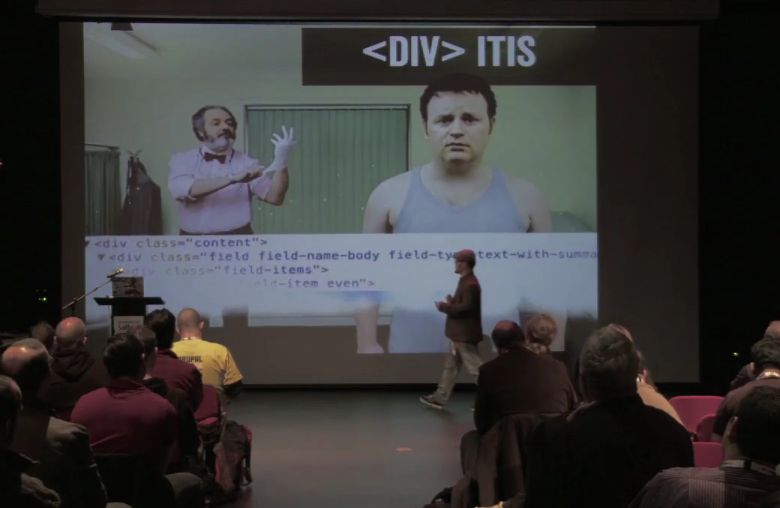
\includegraphics[scale=0.42]{img/online/divitis_morten_dcnw2012.png}
\caption[Screenshot from keynote ``The Angry Themer" at \textit{DrupalCamp} North West 2012]%
{Example of the complaints about ``divitis" from Drupal themers as illustrated during \textit{DrupalCamp} North West 2012 keynote: ``The Angry Themer". Retrieved \nth{10} November 2016, from \url{https://vimeo.com/54387556}, under a CC BY-SA 2.0 license.}
\label{divitis}
\end{figure}

The existence of this tension between division of labour and the object was explained by Drupalistas to be due to a lack of communication between backend and frontend developers. The following excerpt, extracted from the same presentation, illustrates this tension:

\begin{quotation}
``[...] [During a social event in DrupalCon Denver (March, 2012)] I was out on the way to the car, and I was bitching and moaning to webchick [backend developer and core comitter]: `How the fuck? Why don't you give us the markup we want? Why can't I change everything?'. And at some point, I think she just got tired of me, like, looked at me, those kind of eyes, like... `Morten, nobody told us what to do!' And I am like...`Eh? But I have been telling you guys that for years'. [EXPLAINING HER ANSWER] `Well, nobody told anybody in the development community what to do'."
\begin{flushright}\footnotesize{Extracted from \textit{DrupalCamp} North West 2012 keynote: ``The Angry Themer" (14'.58" - 15'.20"). Retrieved \nth{18} November 2016, from \url{https://vimeo.com/54387556}, under a CC BY-SA 2.0 license.}\end{flushright}
\end{quotation}

In the context of the same presentation, this Drupalista also explained the passive role of frontend developers in the early stages:

\begin{quotation}
``[...] Eight years ago there was nobody [referring to the themers], six years ago I think there was just me and one other, ... five years ago we were maybe ten, three years ago in DC [referring to DrupalCon DC (March, 2009)] there was a bunch of us... so this is also a blame on the frontend community, that nobody told anybody in the backend or the development community what is it that we wanted [...] So at this point you can choose two different ways: either you can be bitching and moaning [...] or you can try to figure out how can we work around this."
\begin{flushright}\footnotesize{Extracted from \textit{DrupalCamp} North West 2012 keynote: ``The Angry Themer" (15'.20" - 16'.12"). Retrieved \nth{18} November 2016, from \url{https://vimeo.com/54387556}, under a CC BY-SA 2.0 license.}\end{flushright}
    \end{quotation}

The consequences of this tension between division of labour and the object can be interpreted as generating an ``itch to be scratched" \parencite{torvalds2001just} by themers. As illustrated by the previous quote, some of them started to organise themselves in 2006 \parencite{morten-history:Online}. These initial efforts were firstly discussed and materialised in the \textit{contributed} system, not surprisingly due to the higher degree of flexibility and experimentality which characterises it. This is illustrated, for example, by the development and release in 2009 of modules such as Style Stripper \parencite{styletripper:Online}, or base themes\footnote{A base theme is a basic theme providing a small amount of style which can be used as a wireframe or template to build other themes on top of it \parencite{base-theme:Online}.} such as Mothership \parencite{mothership:Online}, which provided ways to clean up the excessive markup generated by Drupal's theme engine in the themers' eyes, and offered them more control over their work. Hence, an emergent progression towards an active role of frontend developers can be observed. The following excerpt, by I\textunderscript{15}, provides an overview of the emergence of these initiatives in the socio-technical system of \textit{contributed} projects at the time, the more active role taken by some frontend developers, and the relevance of building a reputation through contributions in order to be able to participate in changes in core:

\begin{quotation}
``[...] Drupal 6 [February, 2008] came out, and I remember looking at the theme system: [...] `Why do we have so much markup?!' [...] So eventually I developed a theme called the `Mothership'. First of all, because I learnt that you can bitch and moan about the system as much as you want, but in Open Source talk is pretty much nothing, code is the currency we live by [...] . And there's also a social economy around this. [...] [When you go to a Drupal event] you want to talk about the module you're building, the theme you build, the project you build. That's your currency. [...]"
\begin{flushright}\footnotesize{Drupal frontend developer, M, 10 years.}\end{flushright}
\end{quotation}

While these \textit{contributed} projects provided partial solutions to the problem, themers felt these changes were so relevant that they should be implemented in the heart of Drupal. However, as previously discussed, changes in core are more difficult to achieve because of the high level of legitimacy necessary to perform those changes, the high quality standards and strong peer-reviewing processes, as well as the high level of complexity and interdependency of the object, among other factors. In addition, the degree of the themers' self-organisation was significantly low at the time, and their voices were also less heard in the community \parencite{Zilouchian2011}. The following anecdote reported by I\textunderscript{15}, regarding frontend developers running a parallel set of frontend sessions during DrupalCon DC (March, 2009), depicts the situation at the time:

\begin{quotation}
``[...] There was only two frontend sessions. There was me and \textit{Matthew}, the maintainer of the [core] theme system [...]. Both of us got pissed off: `Why there is only two sessions about the frontend? How can ...? Apparently everything else matters so much more, but actually how sites are built is not relevant from the developer perspective'. [...] So, \textit{Matthew} asked all the people who submitted sessions, and they submitted them to him, and he picked out 20 [frontend rejected] sessions, [...] and he took one of the BoF [Birds of a Feather] whiteboards, and put the whole program and say: `This room in there is the frontend room, and, by the way, you can all go fuck yourselves' [LAUGHS]. That was pretty much the attitude."
\begin{flushright}\footnotesize{Drupal frontend developer, M, 10 years.}\end{flushright}
\end{quotation}

In the context of the same anecdote, I\textunderscript{15} explains how a more empowered group of frontend developers began to emerge:

\begin{quotation}
``[...] Suddenly, I realised it was not only me and \textit{Matthew}: we had a ton of people coming and willing to talk about what to do about this [referring to changing the frontend]. [...] [Months later] I was beginning to know a lot people [...], these connections started to be made, and we came up with an idea: `let's do a frontend conference' [...]"
\begin{flushright}\footnotesize{Drupal frontend developer, M, 10 years.}\end{flushright}
\end{quotation}

During the next years frontend developers started to organise themselves in more regular and formal ways \parencite{d4dgroup:Online}. The emergence of the initiative, as depicted by the previous quote, went beyond the online limits. As observed during my participation and emphasised by all the Drupalistas interviewed about the initiative, F2F events played a significant role in fostering the initiative\footnote{The socio-technical systems of Drupal events are extensively described and analysed in chapters \ref{mostly-offline-local:chapter} and \ref{mostly-offline-cons:chapter}.}. These events, originally known as D4D or Drupal Design Camps emerged in Boston in 2009 \parencite{d4dcamp:Online}, and were extended to Europe in 2010 \parencite{d4dcamp_eur:Online}. In 2012 they were renamed as ``Frontend United" \parencite{fe_united:Online}, one more example of how this increasing sense of empowerment and self-determination was reflected, including in the naming of the events themselves. Picture \ref{frontend-united-2012} depicts the first ``Frontend United" meeting in Amsterdam in April 2012, with more than 200 attendees according to the statistics offered by the event organisers, and picture \ref{frontend-united-symbol} illustrates the use of specific symbology by the group.

\begin{figure}[H]
\centering
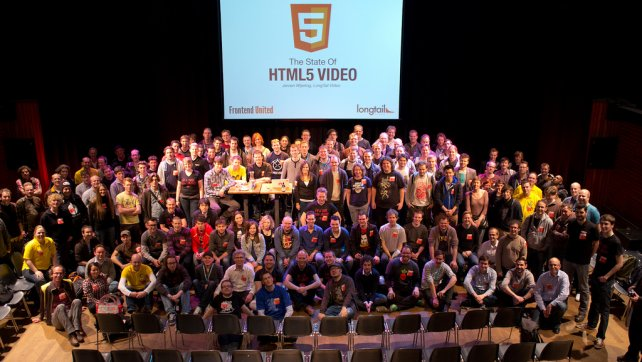
\includegraphics[scale=0.6]{img/online/group-photo_fu_2012.jpg}
\caption[Group photo during Frontend United 2012]%
{Group photo during Frontend United 2012, in Amsterdam. Retrieved \nth{14} November 2016, from \url{https://www.flickr.com/photos/elv/6952927548/in/photostream/}, published by Philippe Gervaise, under a CC-BY-SA license.}
\label{frontend-united-2012}
\end{figure}

\begin{figure}[H]
  \centering
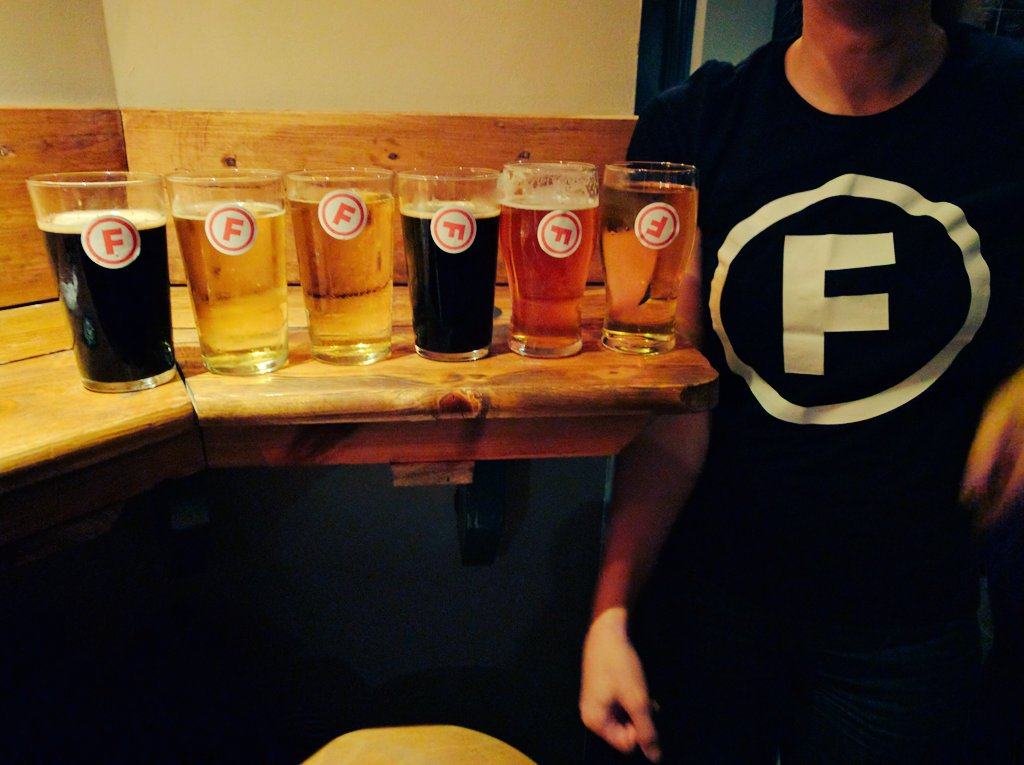
\includegraphics[scale=0.3]{img/online/fe-united-logo.jpeg}
\caption[Picture of a ``Frontend" T-shirt]{An example of the development of symbology for the group of Drupal themers. In this case, a ``F" standing for Frontend. Retrieved \nth{14} November 2016, from \url{https://twitter.com/frontendunited/status/781988434583879680} by @frontendunited.}
\label{frontend-united-symbol}
\end{figure}

With the rise of core initiatives for Drupal 8 presented in section \ref{subsec:dec-form-core}, frontend developers envisioned an opportunity to implement these changes in Drupal's core. They organised themselves around ``Twig in Core", an unofficial core initiative named after the decision to include the FLOSS template engine Twig\footnote{Twig \parencite{twig-doc:Online} is a FLOSS template engine for PHP inspired by Python engines such as Jinja \parencite{jinja:Online} or Django's engine \parencite{django:Online}. It consists of an intermediate layer which allows the effective separation of the presentation layer from the logical one, creating faster and more secure PHP code, and providing more control for template designers, in this case Drupal themers. It is also employed by several popular FLOSS projects such as Symfony, phpBB or Piwig among others.}. The following quote, by I\textunderscript{15}, provides an overview of some of the most relevant events at the time:

\begin{quotation}
``[...] In [Frontend United] Amsterdam [2012], we were doing brainstorms on how the system should work [...] And \textit{Peter} [a well-known Drupal developer who was looking at the issue while attending a parallel Drupal event in San Francisco] came up with the idea of using Twig [...]. And there were 200 frontenders there [in Amsterdam]... and we had no fucking idea what Twig was. But there was this one dude... `I know about Twig, I can do a clone and show you how it can do things more elegant [...]'. So he showed it to us ... and it made a lot of sense, because it made the system more elegant but also secure. It was a kind of match, [...] because for [backend] developers it made the system more secure [implying this is one of the most relevant aspects for them]. [...] So [to include Twig] we would need to write everything: convert every single function into a template. [...] And I was like: `OK, this is good. If we force ourselves to do this, we cannot have Drupal 8 out of the door before we finish all this work'. So, to me, that was a kind of pact with the Devil. [...] And we started having weekly meetings. [...] Several people started jumping in, [...] and we suddenly start to have a small group of people who were showing up every week. [...]"
\begin{flushright}\footnotesize{Drupal frontend developer, M, 10 years.}\end{flushright}
\end{quotation}

These excerpts illustrate the emergence of a more formal and organised group of frontend developers to carry out  these changes in core; hence depicting a progression over time from a passive position, as the one described by \textcite{Zilouchian2011} or the initial period referred to in previous quotes, to an active one. Rather than relying on lobbying techniques \parencite{Zilouchian2011}, they self-organised around an initiative, also including backend developers, to produce these architectural changes in core. This progression can be interpreted as a growing form of self-empowerment of frontend developers in the community.  The following excerpt by a Drupalista who joined the initiative at the time, extracted from a comment on a blog post on authority and FLOSS, provides an overview of this increasing degree of self-empowerment in the group, as well as how decentralisation in decision-making and rotation in leadership characterised the subsequent stages in organisational terms within the initiative:

\begin{figure}[H]
 \centering
 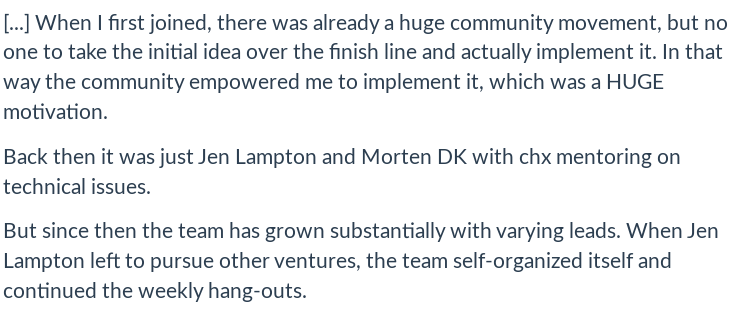
\includegraphics[scale=0.5]{img/quotes_replacement/quote_twig_cc.png}
 \caption[Excerpt (I) from comment in the article ``On authority in Drupal and/or Open Source in general"]{Drupal core committer, M, 4 years. Excerpt (I) from comment in the article ``On authority in Drupal and/or Open Source in general". Retrieved \nth{15} March 2015, from \url{http://hojtsy.hu/blog/2014-oct-17/authority-drupal-andor-open-source-general}, under a CC BY-SA 2.0 license.}
\label{quote_twig_core_01}
\end{figure}

A key moment for the initiative occurred when Twig was committed to core during a \textit{DrupalCamp} in November 2012 \parencite{badcamp2012:Online}. The commit was carried out as a ``live commit", a gathering of Drupalistas during F2F events in which commits are publicly pushed as part of a community celebration, also providing public acknowledgement of contributions. Picture \ref{twig-core} shows the euphoria of one of the main leaders of the initiative during the live commit, a culmination of all the hard work carried out by the initiative up to that point.

\begin{figure}[H]
\centering
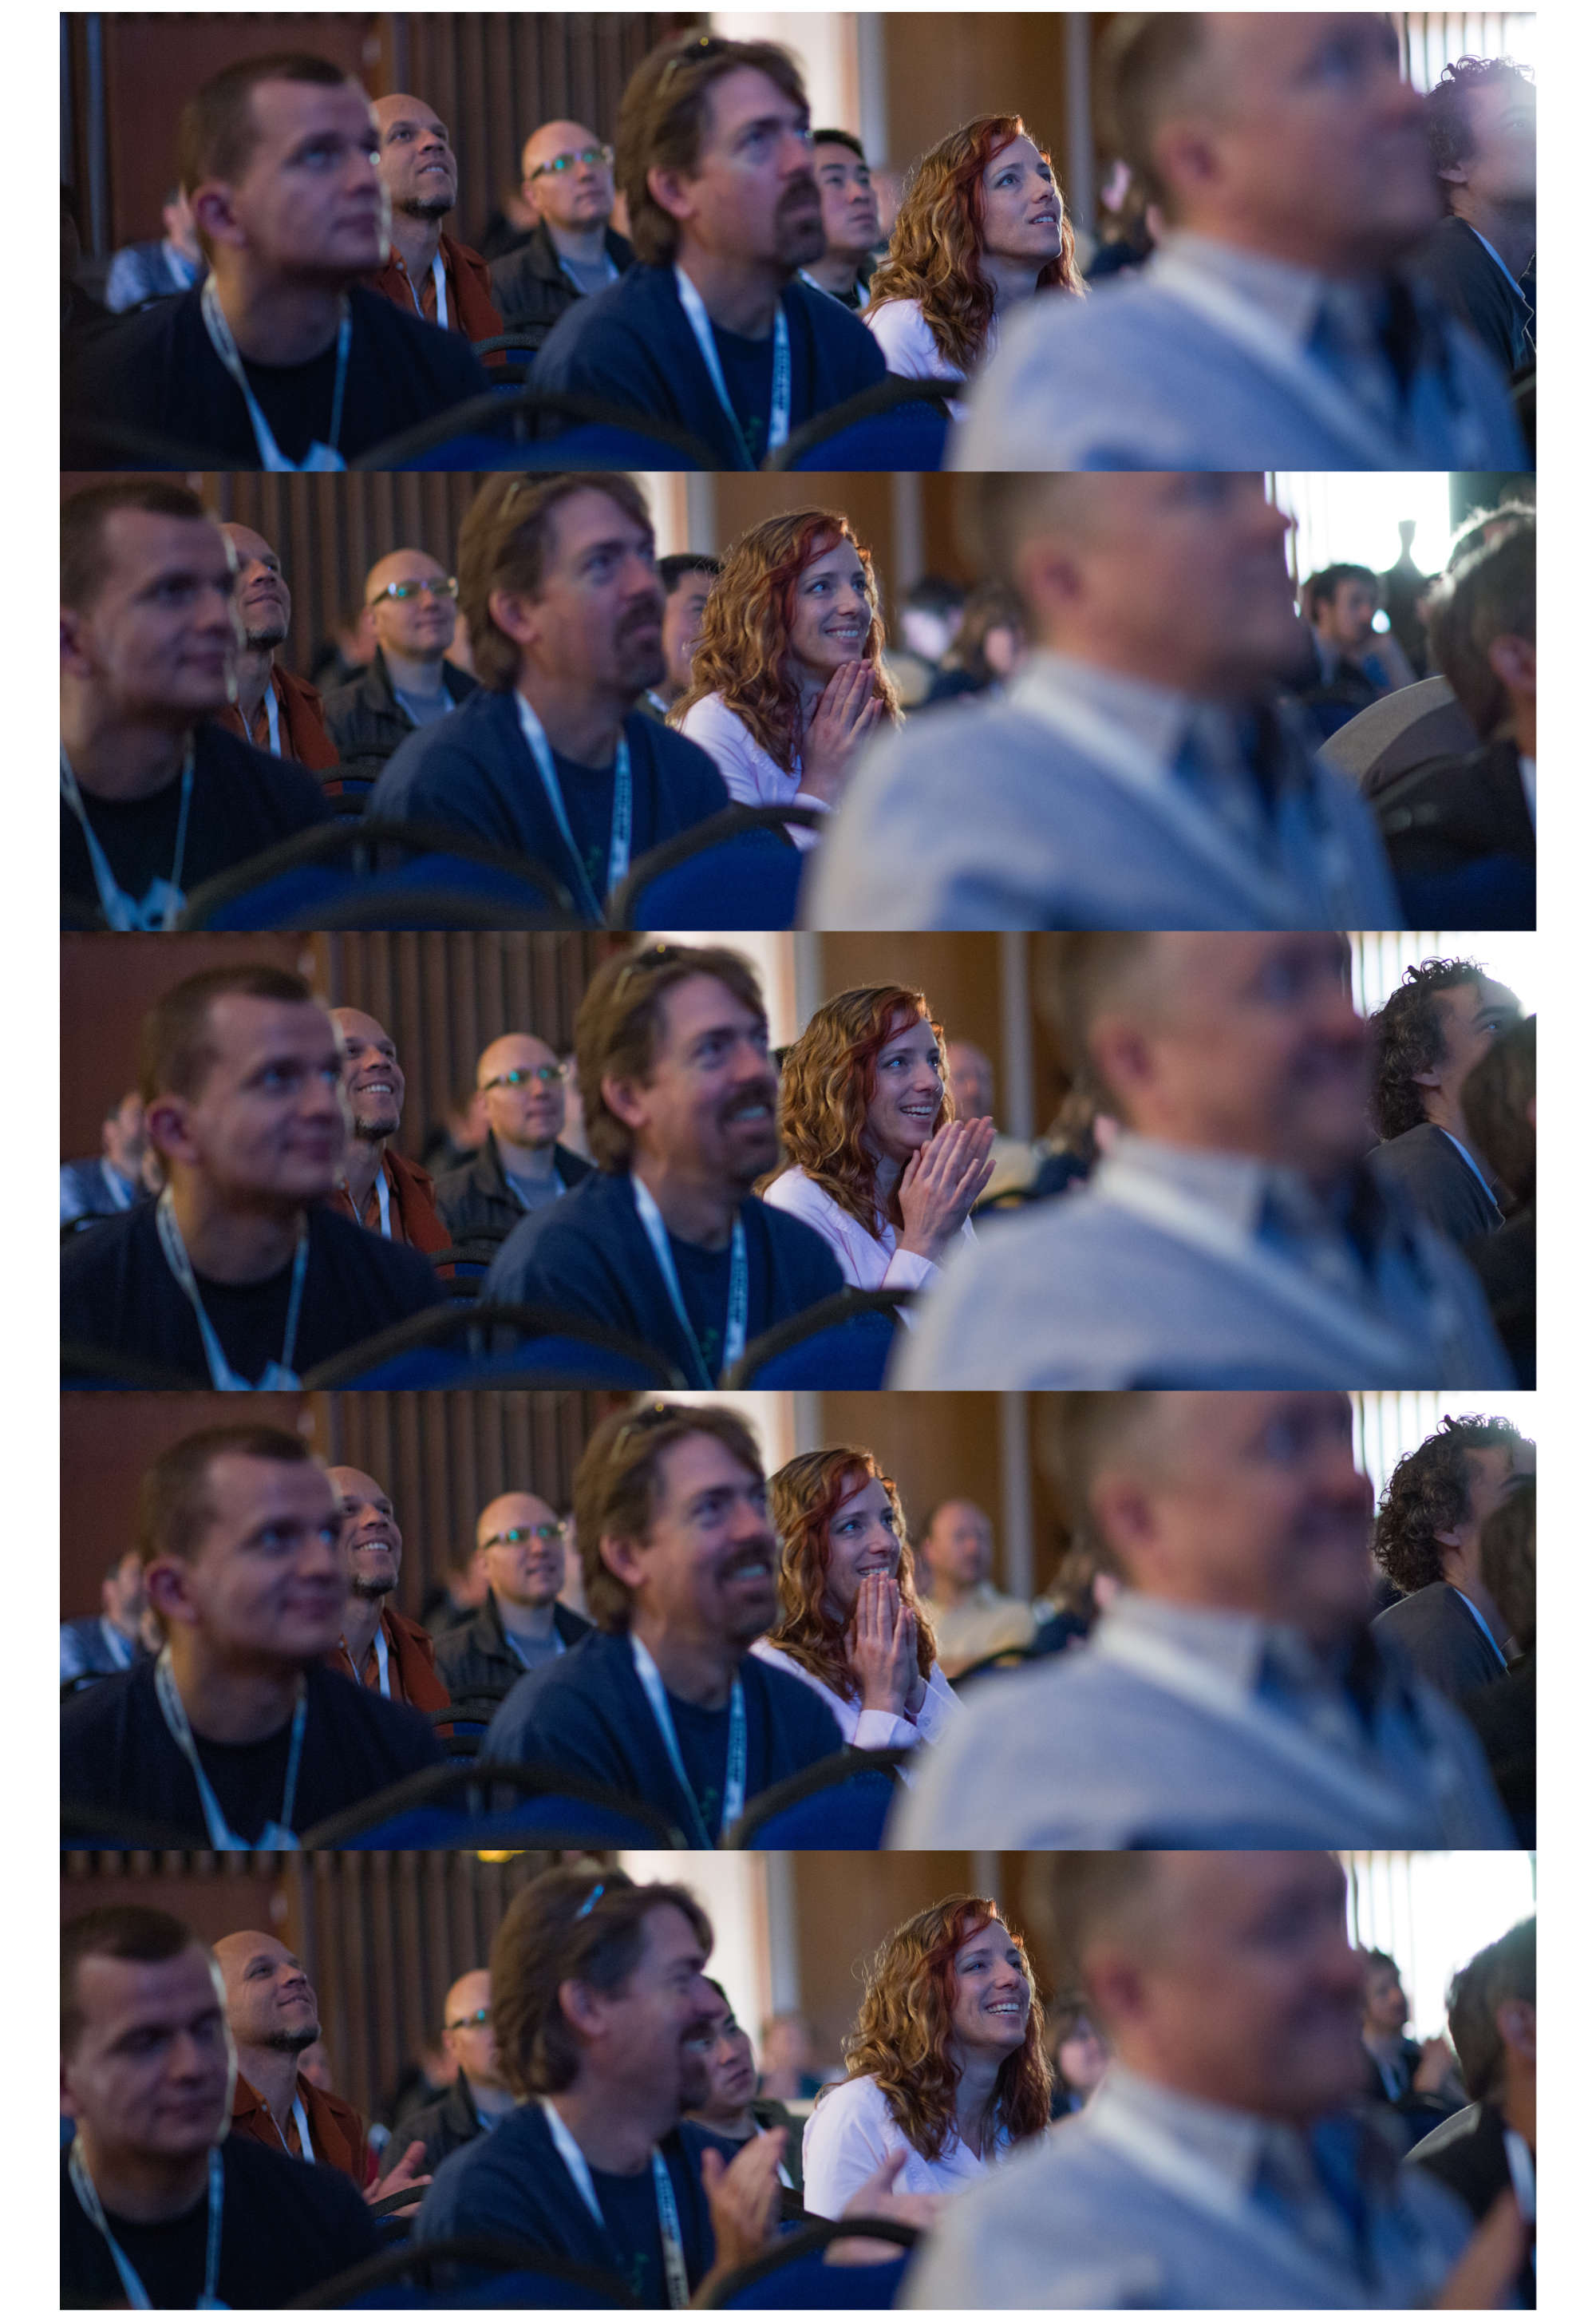
\includegraphics[scale=0.45]{img/online/twig_in_core.jpg}
\caption[Pictures from the committing of ``Twig in Core" during BADCamp 2012]%
{Jen Lampton --- the Drupalista in the middle of the picture joining her hands ---, one of the most visible leaders of the `Twig in Core' initiative at the time, watches as Twig is committed to Drupal core live during the BADCamp 2012. Picture by Ezra Barnett Gildesgame retrieved \nth{22} November 2016, from \url{https://www.flickr.com/photos/ezrabg/8155887186/}, under a CC-BY license.}
\label{twig-core}
\end{figure}

\subsection{Self-organisation, decentralisation and empowerment within a core initiative}

As presented in the previous section, frontend developers progressed from a passive to an active position, and self-empowered and organised themselves to create an initiative which would change the direction of the Drupal project. In the subsequent years, this led to the development of a more formalised group, which in the eyes of some of the participants was even a sub-community within Drupal, as illustrated by the following excerpt by I\textunderscript{15}:

\begin{quotation}
``[...] [Twig in Core] has been pretty much about building a community on the side. We now have this Twig Slack\footnote{See \url{http://drupaltwig-slack.herokuapp.com}.} channel with more than 600 people. That was pretty much the approach: building a community that can help the Drupal community. Because we couldn't build it inside of Drupal, because inside of Drupal... it was so much built on engineering and development. And we wanted to talk design and implementation. [...]"
\begin{flushright}\footnotesize{Drupal frontend developer, M, 10 years.}\end{flushright}
\end{quotation}

This process entailed the development of an environment which facilitated decentralisation of decision-making and fostered a sense of empowerment in the participants, as illustrated by the following excerpt from the interview with I\textunderscript{14}, who became an active member in the initiative at the time and led it for almost a year:

\begin{quotation}
``[...] it was totally a grassroots initiative, it was just people trying to do things better. Especially, if you go later on in Twig in Core in 2013, 2014, and so on, then... what you see is the larger Drupal frontend community behind this thing, and really helping to try to push it forward, even if they're not sure they have the skills to do so, but having the passion, the enthusiasm and the desire to push this change. I think that's how it was successful, it wouldn't have been successful if it was just the same four or five people working on it for years, that's just not enough, it needed a bigger community, it needed that support. [...]"

    \begin{flushright}\footnotesize{Drupal frontend developer, and core committer after the initiative, M, 6 years.}\end{flushright}
    \end{quotation}

During the following years, the initiative evolved within an organisational environment with internal and external tensions, which were reflected in the entities surrounding its organisational processes. On one hand, the high interdependency of the object required an almost full version, since a partial one would make Drupal core unshippable\footnote{The term unshippable, in the context of software development, refers to an unfinished version affecting some of the critical functionalities.}. This was a source of tensions, which at several points brought into question the future sustainability of the initiative, and even the legitimacy of the changes to remain in core. For example, the following excerpt by I\textunderscript{14} illustrates some of these external tensions, in which it was discussed whether Twig should be rolled back:

\begin{quotation}
``[...] in a way we needed to almost sell it to Dries and to the core committers and say: `We know this isn't an official initiative, but, you know, we hope you agree that it's a good thing' [...]. So I met Dries for the first time at DrupalCon Portland [May, 2013], ... and I just remember him asking things like [...]: `If the Twig team went away, would you still want Twig in Core?', like, `Would you still put it in core?'. So I think, there's a lot into that, I think, but part of what he was asking is like: `Is this something that people can and will maintain? Or is it just like your baby that, you know, you're putting into core?' [LAUGHS]. [...] we had to do the work first [...], so in [DrupalCon] Portland [May, 2013] basically what happened is if we didn't meet the deadline, if we didn't have everything go in all at once [...] Drupal would have been in a less shippable state, let's say, because if we would just have converted [the existing templates] one by one, [...] if you end up shipping Drupal with half PHP templates and half Twig... that's not good [LAUGHS]. [...] It needed to be full, kind of comprehensive. Otherwise it would've never worked, and we would've just had to roll it back [...]"

\begin{flushright}\footnotesize{Drupal frontend developer, and core committer after the initiative, M, 6 years.}\end{flushright}
\end{quotation}

On the other hand, there was a lack of consensus at the time within the group regarding the way in which the philosophy of the new theming system should be implemented, also producing internal tensions. A survey\footnote{Unfortunately, no sources could be found regarding the survey design beyond an interview in a Drupal podcast \parencite{twig-morten-interview:Online}. During the interview with I\textunderscript{15}, the Drupalista most heavily involved in the survey design and dissemination, he reported the survey was taken by more than 500 Drupal frontend developers, and it was mainly distributed via social networks and frontend developers channels.} designed and disseminated by the group showed what at the time seemed to be two mutually-irreconcilable positions. On one hand, around a third of the themers who participated in the survey were in favour of a completely clean system, lacking default divs and CSS. On the other hand, the two remaining thirds preferred a system with a cleaner but substantial default amount of them.  A key moment for the group to reach a consensus in the initiative occurred during DrupalCon Austin (June, 2014), in what was known as the ``consensus banana" -- picture \ref{consensus-banana} depicts a picture taken around the famous banana.

\begin{figure}[H]
\centering
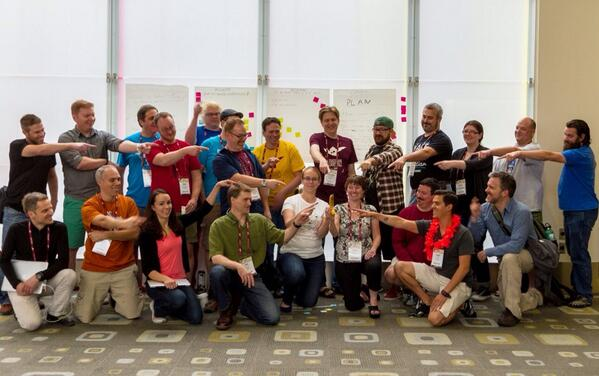
\includegraphics[scale=0.6]{img/polycentric/consensus-banana.jpg}
\caption[Group picture of the participants in the ``consensus banana" BoF at \textit{DrupalCon} Austin 2014]%
{A group picture of the participants in the BoF of the ``consensus banana", another humorous form characteristic of the hacker culture \textcite{coleman2013coding}. Picture retrieved \nth{22} September 2016, from \url{https://www.drupal.org/files/issues/consensus-banana.jpg}.}
\label{consensus-banana}
\end{figure}

The consensus banana refers to a popular story within the Drupal community in which, during a BoF in \textit{DrupalCon} Austin 2014, frontend developers employed a banana as a pointer stick to try to push forward decision-making and reach a point of consensus for the philosophy of the new theming system. That point of consensus was reached by the creation of two themes representing both philosophies: ``classy" and ``stable". The default behaviour of the system would be to reduce the markup as much as possible, drawing on the base theme,``stable", but core would also be shipped with ``classy", another base theme which provides classes to help annotate markup elements. Several outcomes were produced as part of this episode as well, such as a more formalised roadmap for the initiative \parencite{consensus-banana:Online}. The following excerpt, extracted from the same previous comment, summarises this episode and some of its main outcomes:

\begin{figure}[H]
\centering
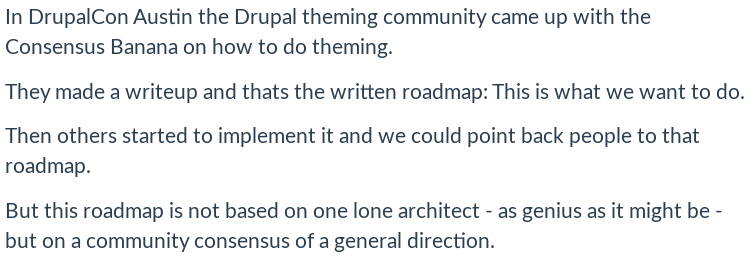
\includegraphics[scale=0.5]{img/quotes_replacement/quote_twig_cc2.png}
 \caption[Excerpt (II) from comment in the article ``On authority in Drupal and/or Open Source in general"]{Drupal core committer, M, 4 years. Excerpt (II) from comment in the article ``On authority in Drupal and/or Open Source in general". Retrieved \nth{15} March 2015, from \url{http://hojtsy.hu/blog/2014-oct-17/authority-drupal-andor-open-source-general}, under a CC BY-SA 2.0 license.}
\label{quote_twig_core_02}
\end{figure}

Beyond the technical issues related to this consensus, the interesting part for this study is in the changes experienced in the organisational processes over time in this core initiative. Under an increasing need to scale up decision-making, a higher degree of formalisation was experienced in the self-organisational processes and reflected in the most relevant entities. For example, a more formalised and explicit set of rules were defined by the group, as illustrated by the creation of the roadmap, the definition of the initiative principles \parencite{twig-core-guidelines:Online}, and the participation through public periodic recorded calls\footnote{See \url{https://www.youtube.com/user/jenlampton/videos} and \url{https://www.youtube.com/channel/UCl51NoedmaLaaZg3pu1jmCQ/videos?shelf_id=0&view=0&sort=dd}.}. Similarly, it was also reflected in the main artefacts employed for collaboration, as depicted by the creation of specific platforms for the initiative --- see figure \ref{drupaltwig} as an example --- and by the usage of surveys to collect feedback from the community.

\begin{figure}[H]
\centering
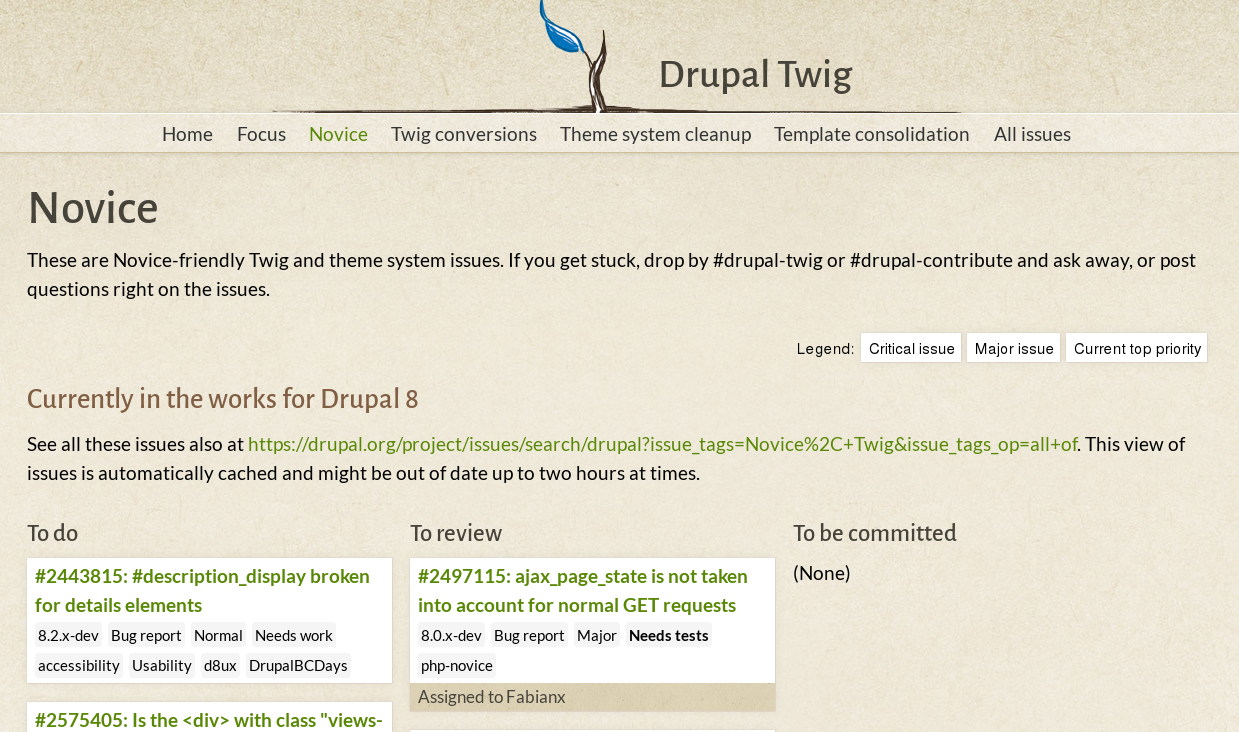
\includegraphics[scale=0.3]{img/online/drupaltwig.png}
\caption[Screenshot of DrupalTwig.org]%
{Partial screenshot of DrupalTwig.org (\url{http://drupaltwig.org/}), depicting the novice section, with issues tagged as novice-friendly. Retrieved \nth{28} November 2016, from \url{http://drupaltwig.org/issues/novice}.}
\label{drupaltwig}
\end{figure}

In addition, formalisation was reflected in the division of labour, as depicted by more explicit roles regarding leadership, which rotated over time, and a more explicit definition of roles for the day-to-day work on the issues. The following quote from the interview with I\textunderscript{13}, who joined the initiative after the `consensus banana' and ended up leading it a year later, depicts some of the main organisational characteristics during this period:

\begin{quotation}
``[...] I got involved at the consensus banana time [March, 2014][...]. In the beginning \textit{Josh} created an agenda, he would have, like, a list of issues to discuss in the call [...]. I started running it in 2015, and we started doing this with a more community approach. Everyone who wanted to participate would create their own, like..., role. So there was a template: `I will be working on these issues, [...]'. And there was another section: `These issues need attention' [...]. So it became a bit more community-oriented and we got more momentum because of that."

\begin{flushright}\footnotesize{Drupal backend and frontend developer, M, 6 years.}\end{flushright}
\end{quotation}

I\textunderscript{13} also explained how this affected decision-making processes, and the distribution of power and rotation in the leadership:

\begin{quotation}
``[...] Obviously it was always very, very consensus-based. Finding consensus isn't always easy, but everything was consensus-based. So there was never only one person making decisions, [...] [those leading the initiative at each point] were not trying to force any issues. [...] We discussed a lot of these things in the meetings, the issue lists... and also the big decisions were done during DrupalCons, [...] and there was definitely rotation [in the leadership]. During each cycle, only maximum of one year, ... less than one year per person who was kind of the person trying to lead the team. [...] There was a very specific core team all time, ... there was new people who got in. [...] The size of the [core] team, in the end became bigger, even if people were leaving that crew, but it was never getting smaller at any point until Drupal 8 got released. [...]"

\begin{flushright}\footnotesize{Drupal backend and frontend developer, M, 6 years.}\end{flushright}
\end{quotation}

The previous excerpt illustrates the existence of a core team within the initiative, in congruence with the common distribution in participation found in many other CBPP communities discussed in section \ref{sec:cbpp-research}; but most importantly, how the initiative was also characterised by a significant degree of rotation in leadership, in which an essential aim was to hear participants' opinions. It can be observed how, within the initiative, power was distributed and loose even from those leading the initiative at previous stages. For example, with regard to decision-making related to the architectural design and philosophy of the new engine, the following excerpt, also extracted from the previous comment by a Drupalista leading the design during the stage before the ``consensus banana", provides an illustration of this distribution of power, rotation and decentralisation of decision-making within the initiative:

\begin{figure}[H]
\centering
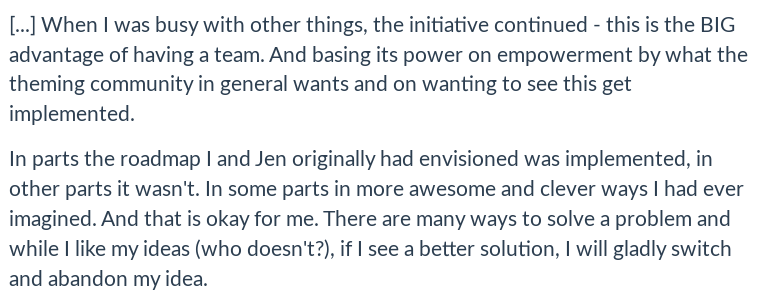
\includegraphics[scale=0.5]{img/quotes_replacement/quote_twig_cc3.png}
 \caption[Excerpt (III) from comment in the article ``On authority in Drupal and/or Open Source in general"]{Drupal core committer, M, 4 years. Excerpt (III) from comment in the article ``On authority in Drupal and/or Open Source in general". Retrieved \nth{15} March 2015, from \url{http://hojtsy.hu/blog/2014-oct-17/authority-drupal-andor-open-source-general}, under a CC BY-SA 2.0 license.}
\label{quote_twig_core_03}
\end{figure}

The analysis of the data collected for the study of this initiative reveals the relevance that the sense of empowerment of frontend developers had to carry out the initiative successfully. The following excerpt, from the interview with I\textunderscript{12}, provides an illustration of this relevance, and how it was extended by, and within, a constantly growing group of frontend developers involved in ``Twig in Core" during this ``post-consensus banana" period:

\begin{quotation}
``[...][in the beginning] it was basically \textit{Jorgen} empowering us... [...] and then we took that message: `We can make the frontend better. We can take this and have the power to improve it!' [...] And \textit{Jorgen} was the main person who went around the World saying it, and then we all did that as well. [...] I don't think an initiative like this would have been possible five years ago, ... there was just not enough of us [frontend developers]. He empowered a few of us, and then we took that, and empowered a handful more people, ten people, it kind of grew from there. And at every event we had more people joining in ... it was incredible. I don't know how all these tables and tables of people [referring to Drupalistas contributing to the initiative during code sprints held at events] ... it just grew over the last few years. [...]"

\begin{flushright}\footnotesize{Drupal frontend developer, F, 4 years.}\end{flushright}
\end{quotation}

\subsection{Release of Drupal 8 and beyond}

The release of Drupal 8 on 19th of November 2015 \parencite{d8-release:Online} represented, among many other major changes in Drupal's core, the culmination of the work carried out by the ``Twig in Core" initiative. After years of work to tackle this  ``scratch to be itched" by frontend developers, the frontend of Drupal was completely changed. The following excerpt, extracted from the abstract of a presentation during the last \textit{DrupalCamp} Florida (March, 2016), shows this sense of fulfilment of the Drupal frontend developers with the changes achieved by the initiative:

\begin{figure}[H]
\centering
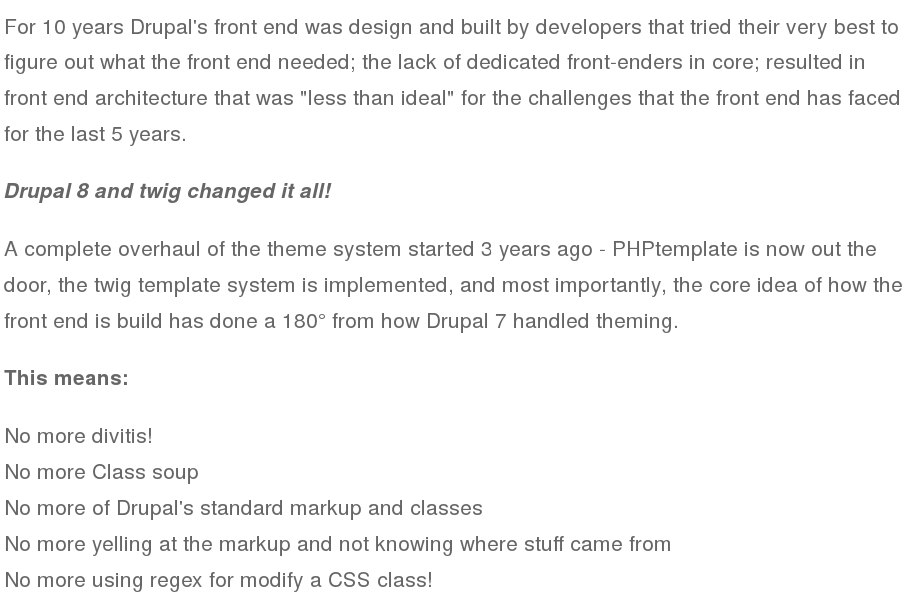
\includegraphics[width=\textwidth]{img/quotes_replacement/dcamp_session_twig.png}
\caption[Excerpt from abstract of session ``Twig \& Drupal 8 Theming" in Florida \textit{DrupalCamp} 2016]{Excerpt from abstract of session ``Twig \& Drupal 8 Theming" in Florida \textit{DrupalCamp} 2016. Retrieved \nth{20} March 2016, from \url{http://2016.fldrupal.camp/sessions/approved/florida-drupalcamp-2016/design-theming-front-end-development/twig-drupal-8-theming/index.html}.}
\label{dcamp_session_twig}
\end{figure}

Beyond the massive technical changes in the object, Drupal core, the previous excerpt also depicts the relevance of the fact that they were driven by those who are most intimately working with this part of the system. Furthermore, when discussing what the most important outcomes achieved by the initiative were with the Drupalistas interviewed, they commonly highlighted the creation of a consolidated group of frontend developers which successfully managed to change the direction of the project, and remains doing so even after the launch of Drupal 8. The following excerpt, from the interview with I\textunderscript{15}, illustrates the relevance of these less visible outcomes in the eyes of Drupalistas:

\begin{quotation}
``[...] creating a place where we could kick that stuff out, and self-organise to build this... it's kind of the ultimate scratch to be itched out. [...] creating a plan, creating a structure, building a community around, bringing in enough people, ... it [the initiative] was way more than creating 600 issues, it was about learning how to organise people around it, [...] now there is a few [frontend] initiatives around. [...] so if you go to our Slack channel [CHECKING THE LINK]... we have 616 users registered on the Twig Slack channel. Of course a lot of them are not active, but that's at least...  that crew means that we have something going on. That it was not completely wrong when \textit{Matthew} took over one BoF room in DC 2009, and said, you know: `We are going to take this over'."

\begin{flushright}\footnotesize{Drupal frontend developer, M, 10 years.}\end{flushright}
\end{quotation}

Overall, this case study illustrates how the dynamics of formalisation and decentralisation that shaped the general organisational processes presented in section \ref{subsec:dec-form-core} operate and materialise at a micro level by carrying out an in-depth study of one of these core initiatives. ``Twig in Core" illustrates how groups of Drupalistas managed to successfully organise themselves to change the global direction of the project. They progressed from a passive position, characterised by requesting changes, to an active one, in which they became accountable for and organised themselves to effectively implement them. As previously presented, the case of this initiative is not unique. While seven official core initiatives were originally proposed by Dries \parencite{d8-official-initiatives:Online}, during the development of Drupal 8 there was a total of 22 initiatives \parencite{d8-all-initiatives:Online}. Although there are differences between these initiatives, for example in their number of participants or whether they were official or not, they all occurred within a general organisational environment which, as depicted in section \ref{subsec:dec-form-core}, tended towards its formalisation, facilitating the decentralisation of decision-making to scale up these processes. Initiatives like ``Twig in Core" should be understood in this context, in which the process of formalisation of some of the entities, such as the rules for whether a project should or should not be part of core, act as an arena to foster initiatives to carry out these changes, in this case even by a group of Drupalistas which had previously had a lesser voice in the community \parencite{Zilouchian2011}. Furthermore, the case illustrates how the aforementioned dynamics also shaped the self-organisational processes of these initiatives. The following quote, in the context of a discussion of the main organisational aspects of these initiatives, shows Dries's views, shared by numerous Drupalistas, on how this degree of decentralisation played a relevant role in the success of the initiatives:

\begin{figure}[H]
\centering
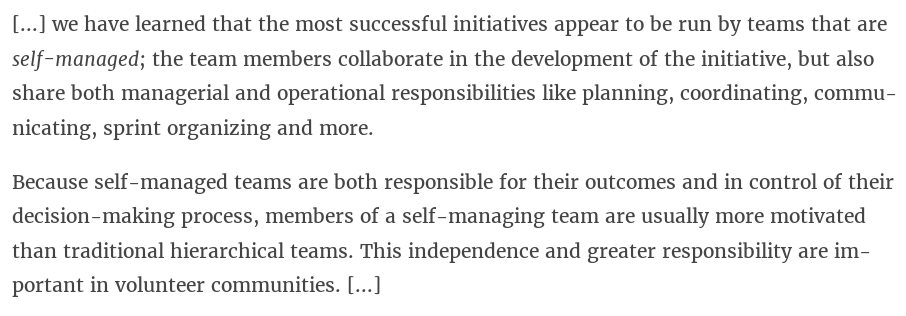
\includegraphics[width=\textwidth]{img/quotes_replacement/power_self_managed_teams.png}
\caption[Excerpt from the article ``The power of self-managed teams in Drupal"]{Excerpt from the article ``The power of self-managed teams in Drupal". Retrieved \nth{3} May 2016, from \url{http://buytaert.net/the-power-of-self-managed-teams-in-drupal}.}
\label{power_self_managed_teams}
\end{figure}

Furthermore, this case study sheds light on the relevance which less visible outcomes had in the life of the community.  As previously illustrated, the outcomes of core initiatives went not only beyond the changes carried out in the object, but they represent the emergence of self-empowered groups which effectively changed these digital commons, following a general dynamic of decentralisation in decision-making even in the most rigid of the socio-technical systems of contribution with respect to the development of projects in the community. As depicted by the previous quote by I\textunderscript{15}, the process continues, and the emergence of these hubs of coordination are already defining the future of Drupal 9's core, through new core initiatives \parencite{d8-new-initiatives:Online}, some of them \parencite{d8-new-theme-in-core:Online} focussed on frontend issues as in the case of ``Twig in Core".

\section{Conclusion}
\label{mosly-online-discussion}

This chapter explored the emergence and main organisational changes of the socio-technical system of \textit{core} projects, the technical heart of the Drupal project. Overall, these changes resulted in a socio-technical system shaped by a ``do-ocratic" culture and characterised by a high degree of perceived internal value of the contributions made to these digital commons, whose quality assurance processes are the most strict and formalised of those identified for ``mostly-online" contribution activities, and changes to which require the highest degree of legitimacy in the eyes of the community, since they affect the general direction of the project.

Subsequently, it was explored how the general dynamics of formalisation and decentralisation operated at a macro level in this socio-technical system, as reflected, for example, in the division of labour, rules and main artefacts employed for collaboration; and how this was intertwined with a general trend towards decentralisation in the decision-making similar to that explained for the case of \textit{contributed} projects, although resulting in a socio-technical system that remained more centralised and with a lower degree of autonomy when compared with that of \textit{contributed} projects.

Finally, the focus was placed on how the aforementioned dynamics operated at a more micro level by exploring a core initiative, showing how these dynamics of formalisation and decentralisation are intertwined in the day-to-day, resulting in a more structured group in which the aim was to hear all participants' opinions and leadership was under rotation. Furthermore, this case study also illustrated the connection between the changes experienced in the general organisational aspects, at a macro level, with the emergence of initiatives themselves at a micro level, illustrating how they provided a scenario that facilitated the empowerment of a group of Drupalistas, whose voices had traditionally been less heard, to change the direction of the project.

Having explored all different socio-technical systems of contribution focussed on the development of projects on the ``mostly-online" side of the spectrum regarding the main medium, a similar approach will be followed over the course of the next two chapters but focussed instead on the exploration of ``mostly-offline" activities: the organisation of Drupal events. The aim now is to explore how the general dynamics of formalisation and decentralisation shaped the overall project; despite the focus of the following socio-technical systems of contribution being on different activities, the development of projects and the organisation of events, and being on the opposite side of the online/offline spectrum with regards to the main medium.